\chapter{Router sin QoS}
\label{chap:sinqos}

\section{Longitud de cola del router}

\subsection{Ejercicio 1.1.1}

\renewcommand{\theenumi}{\alph{enumi}}
\begin{enumerate}
    \item Tasa de entrada [pkt/s] a la cola.

\[
\label{eq:sinqos_tasa_entrada}
R_{in} = R_{VoIP} + 2 \cdot R_{UDP} = \frac{1~\mathrm{pkts}}{20~\text{ms}} + 2 \cdot \left(\frac{1 ~ \text{pkts} }{80 ~ \text{ms} }\right) = \frac{1~\mathrm{pkt}}{0,02~\text{s}} + \frac{2~\mathrm{pkt}}{0,08~\text{s}} = 50 ~ \text{pkt/s} + 25 ~ \text{pkt/s} = 75 ~ \text{pkt/s}
\]

    \item Proporción de paquetes de cada tipo en la cola.

    En VoIp: \[ \frac{R_{VoIP}}{R_{in}} = \frac{50~\text{pkts/s}}{75~\text{pkts/s}} = \frac{2~\text{pkts/s}}{3~\text{pkts/s}}  \approx 66,66\%\]

    En UDP: \[ \frac{R_{VoIP}}{R_{in}} = \frac{25~\text{pkts/s}}{75~\text{pkts/s}} = \frac{1~\text{pkts/s}}{3~\text{pkt/s}} \approx 33,33\% \] 
            (ambos transmisores UDP, cada uno tiene una proporción de \( 16,67\% \)).

    \item Tasa de salida [pkt/s] de la cola, asumiendo que la cabecera del protocolo PPP tiene 7B.
 
    Como está la cabecera PPP de 7B, los paquetes VoIP tendría una cabecera total de 199B y los paquetes UDP una cabecera de 1000B.

    \begin{eqnarray}
        \label{eq:senqos_tasa_salida}
        128~\text{kb/s} \cdot \frac{1000~\text{b}}{1~\text{kb}} \cdot \frac{1~\text{B}}{8~\text{b}} = 16000~\text{B/s} \\
        R_{out} = \frac{16000~\text{B/s}}{ \frac{2}{3} \cdot  199~\text{B/pkts} + \frac{1}{3} \cdot 1000~\text{B/pkts}} = 34,33~\text{pkts/s}
    \end{eqnarray}


    \item ¿Cuánto tarda en llenarse la cola?
    
    Como se ve en la gráfica tamaño de la cola sin QoS, tiene un tamaño de 100pkts:

    \[
    \label{eq:sinqos_tiempo_llenado}
      T_{fill} = \frac{L}{R_{fill}} = \frac{L}{R_{in} - R_{out}} \frac{100~\text{pkts}}{75~\text{pkt/s} - 34,33~\text{pkts/s}} = 2,46~\text{s}
    \]


\end{enumerate}

\subsection{Ejercicio 1.1.2}
La tasa de entrada al dejar de transmitir los paquetes de VoIP, solamente se transmiten los paquetes UDP, entonces en la ecuación \ref{eq:sinqos_tasa_entrada},
solo tendríamos en cuenta la tasa de los paquetes UDP, quedando en:
    
\[
  R_{in} = R_{UDP1} + R_{UDP2} = \frac{1~\mathrm{pkts}}{80~\mathrm{ms}} + \frac{1~\mathrm{pkts}}{80~\mathrm{ms}} = 12,5~\mathrm{pkts/s} + 12,5~\mathrm{pkts/s} = 25~\mathrm{pkts/s}
\]

La tasa de salida, aunque dejemos de transmitir paquetes VoIP, según la ecuación \ref{eq:sinqos_tiempo_llenado}, la cola se llena a los 2,46 segundos
por lo que después de 60s (cuando se deja de transmitir VoIP), la cola seguirá llena entonces la tasa de salida sigue siendo igual hasta que 
se empiece a vaciar.

La consecuencia de tener estas nuevas tasas es que la cola se va a vaciar, ya que: \[R_{in} < R_{out}\]
Una vez pasado un tiempo, la tasa de salida va a ser:

\[
  128~\text{kb/s} \cdot \frac{1000~\text{b}}{1~\text{kb}} \cdot \frac{1~\text{B}}{8~\text{b}} = 16000~\text{B/s} \\
  R_{out} = \frac{16000~\text{B/s}}{1000~\text{B/pkts}} = 16~\text{pkts/s}
\]

En ese momento, al ser la tasa de entrada más grande que la tasa de salida, se va a volver a llenar la cola. Este problema se puede observar
en la gráfica \ref{fig:sinqos_tam}.

\begin{figure}[!ht]
    \centering
    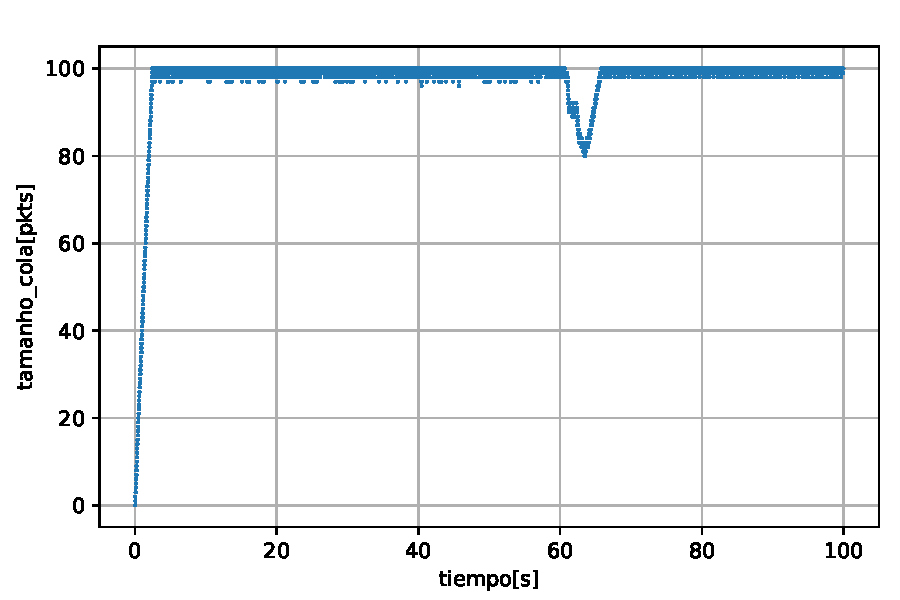
\includegraphics{graficas/sinQoS/tamanho_cola_sinQoS.pdf}
    \caption{Longitud de la cola del router sin QoS}
    \label{fig:sinqos_tam}
\end{figure}

\subsection{Ejercicio 1.1.3}

Estas dos tasas ya se han calculado en el siguiente apartado. Por lo tanto quedaría que:

\[
  R_{in} = 25~\mathrm{pkts/s}
\]

\[
  R_{out} = 16~\mathrm{pkts/s}
\]

\subsection{Ejercicio 1.1.4}

Aprovechando la ecuación para calcular la tasa de salida:

\begin{equation}
    \begin{aligned}
      R_{out} &= 25~\mathrm{pkts/s} = \frac{16000~\mathrm{B/s}}{ x \cdot 199~\mathrm{B/pkts} + (1 - x) \cdot 1000~\mathrm{B/pkts}} \\
      25 &= \frac{16000}{ 199 \cdot x + 1000 - 1000 \cdot x} \\
      25 &= \frac{16000}{1000 - 801 \cdot x} \\
      (1000 - 801 \cdot x) \cdot 25 &= 16000 \\
      25000 - 20025 \cdot x &= 16000 \\
      x &= \frac{16000 - 25000}{-20025} \\
      x &\approx 0,45
    \end{aligned}
\end{equation}

De esta manera, la proporcion de los paquetes VoIP es de 45 paquetes y en el caso de los paquetes UDP es de 55 paquetes, por lo que
nos quedaria un hueco de para 45 paquetes al dejar de transmitir VoIP y no se llenaria la cola

\section{Tiempo en cola del router}

\subsection{Ejercicio 1.2.1}
\begin{enumerate}
    
    \item Calcula el tiempo medio en cola de un paquete cuando la cola está llena: \label{item:a}
    
    Cuando la cola está llena tiene 100 paquetes, por lo que el tiempo medio es de:
        \[
          t_{q} = \frac{L}{R_{out}} = \frac{100~\mathrm{pkt}}{34,33~\mathrm{pkts/s}} = 2,91~\mathrm{s}
        \]
    
    \item ¿A qué se deben las oscilaciones de la gráfica en torno a este valor medio? \label{item:b}
    
    \begin{figure}[!ht]
        \centering
        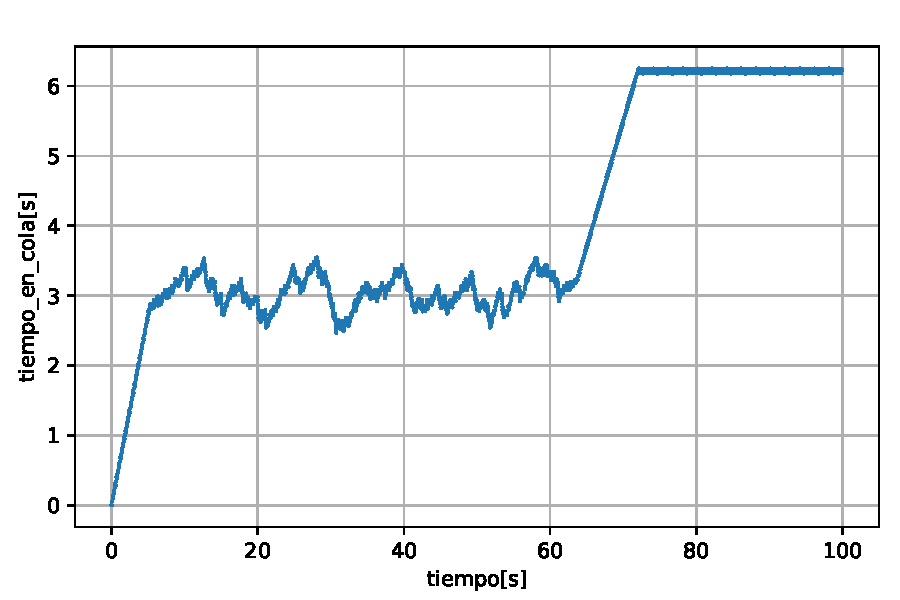
\includegraphics{graficas/sinQoS/tiempo_en_cola_sinQoS.pdf}
        \caption{Tiempo paquetes en cola del router sin QoS}
        \label{fig:sinqos_time}
    \end{figure}

    Como se puede ver en la gráfica \ref{fig:sinqos_time}, hay una oscilación hasta los 60 segundos ya que es cuando se dejan de transmitir los paquetes VoIP. Esa oscilación
    se debe a que los paquetes de voz son mas ligeros que los de UDP, por lo que, hay momentos en que la cola se atasca más ya que a lo
    mejor está liberando los paquetes UDP y otras veces hay una bajada ya que están saliendo los paquetes VoIP
    
    \item ¿Cuál sería la máxima longitud de cola si queremos que el tiempo de encolado de un paquete sea como máximo 1s? \label{item:c}
    
    Para eso vamos a utilizar la ecuación del apartado \ref{item:a}:

    \[
      t_{q} =  \frac{L}{R_{out}} \Rightarrow 1~\mathrm{s} \cdot 34,33~\mathrm{pkts/s} = L \Rightarrow L \approx 35~\mathrm{pkt}
    \]

    Por lo tanto con 35 paquetes como tamaño de la cola, tendremos un encolado de como máximo 1s


\end{enumerate}

\subsection{Ejercicio 1.2.2}
\begin{enumerate}
    
    \item Calcula el tiempo medio en cola de un paquete cuando la cola está llena.
    
    Cuando se deja transmitir VoIP, la tasa de salida de la cola es de:
    \[
      R_{out} = \frac{16000~\text{B/s}}{1000~\text{B/pkts}} = 16~\text{pkts/s}
    \]

    Por lo que el tiempo medio cuando la cola está llena y solo se transmite UDP:
    \[
      t_{q} = \frac{L}{R_{out}} = \frac{100~\mathrm{pkt}}{16~\mathrm{pkts/s}} = 6,25~\mathrm{s}
    \]

    \item ¿Por qué ahora la gráfica no presenta oscilaciones en torno al valor medio?
    
    Como vimos en la gráfica \ref{fig:sinqos_time}, después de 60s (tiempo que solo hay paquetes UDP), no hay ninguna oscilación
    ya que los paquetes son todos de igual tamaño por lo que todos tardan el mismo tiempo en enviarse.
  

\end{enumerate}


\section{Retardo de extremo a extremo}

\subsection{Ejercicio 1.3.1}

\begin{figure}[!ht]
    \centering
    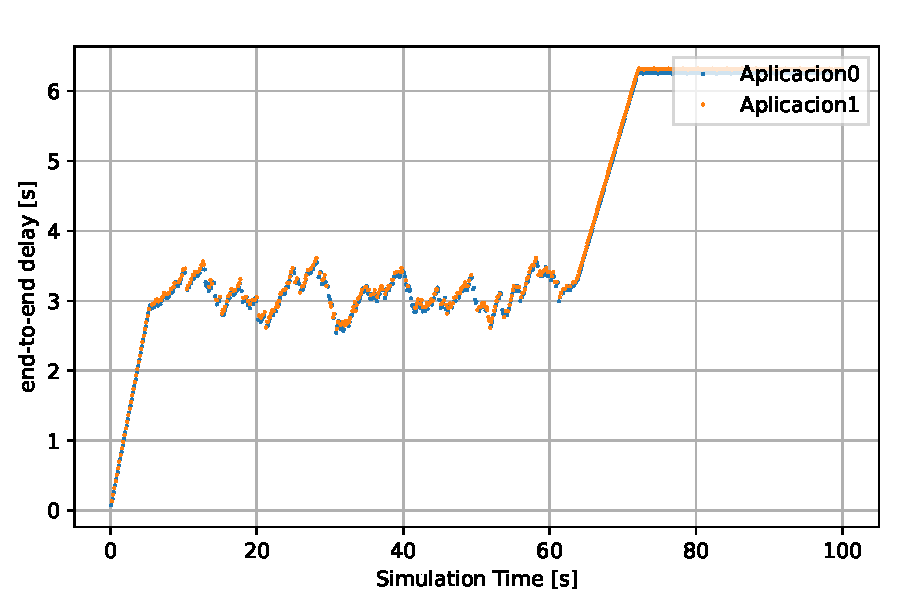
\includegraphics{graficas/sinQoS/ end_to_end__delay_sinQoS.pdf}
    \caption{Retardo extremo a extremos del router sin QoS}
    \label{fig:sinqos_endtoend}
\end{figure}

Hay una relación con el retardo extremo a extremo (tiempo que tarda en llegar los paquetes al destino), con respeto al tiempo de encolado
de paquetes ya que, si los paquetes pasan mucho tiempo dentro de la cola, aumenta el tiempo de llegada de esos paquetes al detini, por lo que
coinciden de una forma similar los tiempos de la gráfica \ref{fig:sinqos_time} con respeto a la gráfica \ref{fig:sinqos_endtoend}


\section{Muestras VoIP y Paquetes VoIP perdidos}

\subsection{Ejercicio 1.4.1}